%!TEX root = ../thesis.tex
\documentclass[..thesis.tex]{subfiles}

\begin{document}

\TODO{Ideas from Nitsan Wakart: https://www.youtube.com/watch?v=pXV4pY42FtM}


Sampling profilers gather call traces from the observable program at regular intervals. Distribution of the gathered samples highlights the hotspots in the observable program. Higher frequency of a call trace suggests that more program's execution time was spent in that particular state. Profiling result is a statistical approximation of the program's performance. Thus, having more samples will provide a more accurate approximation. This approach also assumes that samples are gathered randomly as bias in the samples could potentially yield inaccurate results. 
\TODO{Show a flamegraph to clarify this point?}

\subsection{Sampling profiling biases}
There are multiple problems that the implementations of the sampling profilers could experience.
\subsubsection{Periodicity bias}
This problem occurs when the sampling interval catches on to some program's routine which executions match the sampling interval. Figure ~\ref{fig:periodicityBias} on page ~\pageref{fig:periodicityBias} illustrates the issue behing the bias. Suppose that the observable program runs \texttt{Method X} and \texttt{Method Y} alternatingly for some constant time period. If the dotted lines are the marks for the call trace samples taken during profiling, the results would be skewed as not a single sample represents \texttt{Method Y} in the results.

\begin{figure}[H]
\centering
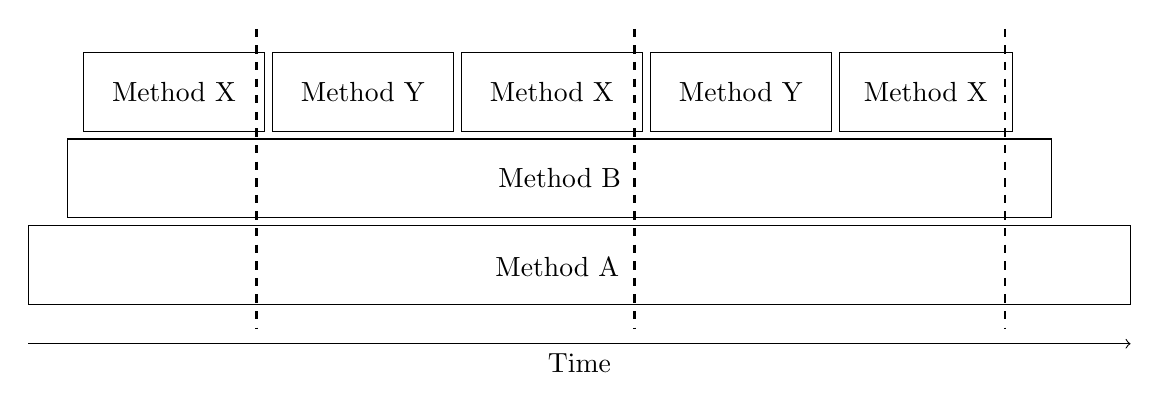
\begin{tikzpicture}
% Call stack rectangles
\draw (0,0) rectangle (14,1) node[pos=.48] {Method A};
\draw (0.5,1.1) rectangle (13,2.1) node[pos=.5] {Method B};
\draw (0.7,2.2) rectangle (3,3.2) node[pos=.5] {Method X};
\draw (3.1,2.2) rectangle (5.4,3.2) node[pos=.5] {Method Y};
\draw (5.5,2.2) rectangle (7.8,3.2) node[pos=.5] {Method X};
\draw (7.9,2.2) rectangle (10.2,3.2) node[pos=.5] {Method Y};
\draw (10.3,2.2) rectangle (12.5,3.2) node[pos=.5] {Method X};

% x-axis time arrow below
\draw[->] (0,-0.5) -- (14, -0.5) node[below, pos=.5] {Time};

% samples
\draw[dashed, thick] (2.9,3.5) -- (2.9,-0.3);
\draw[dashed, thick] (7.7,3.5) -- (7.7,-0.3);
\draw[dashed, thick] (12.4,3.5) -- (12.4,-0.3);

\end{tikzpicture}
\caption{Illustration of periodicity bias}
\label{fig:periodicityBias}
\end{figure}


Possible ways to tackle this problem would be to randomize the sampling interval by having a random number of time units offseting the sampling interval.
\subsubsection{Safepoint bias}
\TODO{Assumption is that samples are taken randomly (referring to safe spots casting a shade on the randomness assumption)}
\TODO{Needs rewording}
As mentioned previously, sampling profiling assumes that the samples are random in a sense that no sample should have a higher chance of occurring than any other sample. When gathering samples from a program running on the JVM, one must take \textit{safepoints} into consideration.

OpenJDK's glossary \cite{jdk_glossary} defines \textit{safepoint} as follows: 
\begin{quote}
A point during program execution at which all GC roots are known and all heap object contents are consistent. From a global point of view, all threads must block at a safepoint before the GC can run. (As a special case, threads running JNI code can continue to run, because they use only handles. During a safepoint they must block instead of loading the contents of the handle.) From a local point of view, a safepoint is a distinguished point in a block of code where the executing thread may block for the GC. Most call sites qualify as safepoints. There are strong invariants which hold true at every safepoint, which may be disregarded at non-safepoints. Both compiled Java code and C/C++ code be optimized between safepoints, but less so across safepoints. The JIT compiler emits a GC map at each safepoint. C/C++ code in the VM uses stylized macro-based conventions (e.g., TRAPS) to mark potential safepoints.
\end{quote}

Safepoints are not precisely documented in the language specifications as they are implementation details of the JVM and each JVM implementation may interpret safepoints differently but they generally work in a similar manner. \TODO{Citation needed}


Some points to expand on
\begin{enumerate}
	\item JVM raises a flag to notify threads to stop on safepoint and then waits the threads to stop on a safepoint. Thread polls for safepoint flag after every 2 bytecode instructions (when in interpreter), end of non-counted loop, method exit, JNI call exit(C1/C2 compiled code), 
\end{enumerate}
\begin{quote}
At a safepoint the thread's representation of it's Java machine state is well described, and can be safely manipulated and observed by other threads in the JVM. - Gil Tene
\end{quote}

\subsection{Sampling profiling possible implementations for the JVM}



\subsubsection{\texttt{AsyncGetCallTrace} profilers}
These kind of profilers make use of an undocumented JVM method \texttt{Async\-Get\-Call\-Trace} \cite{agct_source} which enables obtaining call traces from a thread without the safepoint bias. Due to this characteristic, profiling samples tend to be more 'honest' since the JVM does not have to stop on a safepoint in order to obtain the call trace of the running thread.

Notable examples of such profilers are Honest Profiler and Java Mission Control. \TODO{Citation needed}

Points to expand on:
\begin{enumerate}
	\item Sends interrupt signal to thread and then runs signal handler to collect the stack trace. Only interrupted thread is stopped.
	\item Does not require the thread to be stopped on a safepoint.
	\item Shows only Java stack. (Most problems can be solved on Java level - Nitsan Wakart)
	\item Only operations on CPU are sampled. Blocking/concurrency issues won't be spotted.
\end{enumerate}

\TODO{Pros and cons}


\subsubsection{\texttt{GetStackTrace} profilers}
This method uses function from the official JVM Tooling Interface API \cite{jvmti_doc} called \texttt{GetStackTrace}.

Some points to expand on:
\begin{enumerate}
	\item Safepoint biased. Requires all the threads to be stopped on a safepoint in order top collect call traces
	\item Has higher overhead when compared to other methods. Application having many threads might take a long time for all the threads to reach a safepoint.
\end{enumerate}

\subsubsection{Native profilers}
\subsubsection{\texttt{jstack}}



\end{document}